% % % % % % % % % % % % % % % % % % % % % % % % % % % % % % % % % % % % % % % % % % % %
%                                                                                     %
% Short Sectioned Assignment LaTeX Template Version 1.0 (5/5/12)                      %
% This template has been downloaded from: http://www.LaTeXTemplates.com               %
%                                                                                     %
% Original author:  Frits Wenneker (http://www.howtotex.com)                          %
%                                                                                     %
% Modified by: Fco Javier Sueza Rodríguez (fcosueza@disroot.org)                      %
%                                                                                     %
% Changes:                                                                            %
%	    - Custom Chapters, Sections and Subsections (titlesec package)                %
%           - Document type scrbook (oneside)                                         %
%           - Use babel-lang-spanish package and marvosym                             %
%           - Use hyperref, enumitem, tcolorbox and glossaries packages               %
%           - Use Time New Roman (mathptmx), Helvetic and Courier fonts               %
%                                                                                     %
% License: CC BY-NC-SA 3.0 (http://creativecommons.org/licenses/by-nc-sa/3.0/)        %
%                                                                                     %
% % % % % % % % % % % % % % % % % % % % % % % % % % % % % % % % % % % % % % % % % % % %

%-----------------------------------------------%
%	              Packages                  %
%-----------------------------------------------%

\documentclass[paper=a4, fontsize=11pt, oneside]{scrbook}

% ---- Text Input/Output ----- %

\usepackage[T1]{fontenc}
\usepackage[utf8]{inputenc}
\usepackage{mathptmx}
\usepackage[scaled=.92]{helvet}
\usepackage{courier}
\usepackage[indent=12pt]{parskip}

\usepackage{geometry}
\geometry{verbose,tmargin=3cm,bmargin=3cm,lmargin=2.6cm,rmargin=2.6cm}

% ---- Language ----- %

\usepackage[spanish]{babel}
\usepackage{marvosym}

% ---- Another packages ---- %

\usepackage{amsmath,amsfonts,amsthm}
\usepackage{graphics,graphicx}
\usepackage{titlesec}
\usepackage{fancyhdr}
\usepackage{tcolorbox}
\usepackage{hyperref}
\usepackage{enumitem}
\usepackage[automake]{glossaries}

%--------------------------------------------------------------------%
%                      Customizing Document                          %
%--------------------------------------------------------------------%


% ----------- Custom Chapters, Sections and Subsections -------------- %

\titleformat{\chapter}[display]
			{\bfseries\Huge}
			{Tema \ \thechapter} {0.5ex}
			{\vspace{1ex}\centering}

\titleformat{\section}[hang]
			{\bfseries\Large}
			{\thesection}{0.5em}{}

\titleformat{\subsection}[hang]
			{\bfseries\large}
			{\thesubsection}{0.5em}{}

\titleformat{\subsubsection}[hang]
			{\bfseries\large}
			{\thesubsubsection}{0.5em}{}

\hypersetup{
    colorlinks=true,
    linkcolor=black,
    urlcolor=magenta
}

% ------------------- Custom heaaders and footers ------------------- %

\pagestyle{fancyplain}

\fancyhead[]{}
\fancyfoot[L]{}
\fancyfoot[C]{}
\fancyfoot[R]{\thepage}

\renewcommand{\headrulewidth}{0pt} % Remove header underlines
\renewcommand{\footrulewidth}{0pt} % Remove footer underlines

\setlength{\headheight}{13.6pt} % Customize the height of the header

% --------- Numbering equations, figures and tables ----------------- %

\numberwithin{equation}{section} % Number equations within sections
\numberwithin{figure}{section} % Number figures within sections
\numberwithin{table}{section} % Number tables within sections

% ------------------------ New Commands ----------------------------- %

\newcommand{\horrule}[1]{\rule{\linewidth}{#1}} % Create horizontal rule command


%----------------------------------------------------------------------------------------
%	TÍTULO Y DATOS DEL ALUMNO
%----------------------------------------------------------------------------------------

\title{
\vspace{10ex}
\normalfont \normalsize
\Huge \textbf{Tarea 3: Análisis y Diseño de Redes}
}
\author{Francisco Javier Sueza Rodríguez}
\date{\normalsize\today}

%----------------------------------------------------------------------------------------
%                                     DOCUMENTO
%----------------------------------------------------------------------------------------
\begin{document}

\maketitle

\thispagestyle{empty}

\vspace{68ex}

\begin{center}
    \begin{tabular}{l l}
        \textbf{Centro}: & IES Aguadulce \\
        \textbf{Ciclo Formativo}: & Desarrollo Aplicaciones Web (Distancia)\\
        \textbf{Asignatura}: & Sistemas Informáticos\\
        \textbf{Tema}: & Tema 3 -  Redes de Ordenadores\\
    \end{tabular}
\end{center}

\newpage

\tableofcontents

\vspace{15ex}

\hrule

\vspace{10ex}

\listoffigures

\newpage

\section{Caso Práctico}
Antonio y Juan han sido nombrados responsables del área de sistemas y redes de la nueva empresa AguadulSoft.

La semana pasada tuvieron una reunión con Ada en la que se les comunicó que tendrían que encargarse de proyectos de implantación de redes en oficinas de clientes. Su primer trabajo será un proyecto pequeño para una biblioteca/centro lúdico de una pequeña población cercana. Antes de lanzarse a dicha tarea van a repasar algunos conceptos básicos de redes.

\section{Actividades}

\subsection{Actividad 1: Medios de Trans}

Para esta actividad debes realizar dos tablas con información obtenida en Internet o en los contenidos de la unidad sobre los siguientes medios de transmisión:misión

\subsubsection*{Parte A: Medios Guiados}
Recientemente, el estándar cableado Ethernet de 2.5 Gbps sobre cable de par trenzado está ganando popularidad. Buscando información en Internet, haz una tabla que incluya lo siguiente:

\begin{figure}[H]
    \centering
    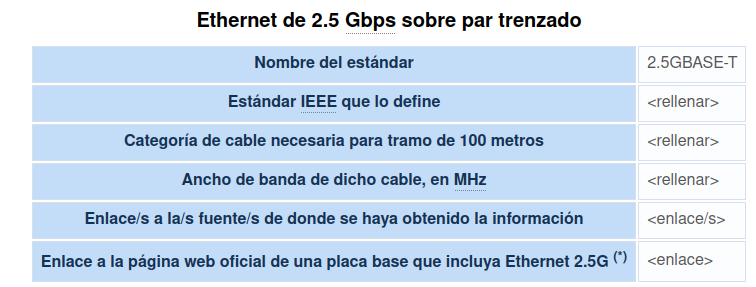
\includegraphics[scale=0.45]{tabla-eth.png}
    \caption{Tabla a completar con datos de la interfaz Ethernet}
\end{figure}

\subsubsection*{Parte B: Medios inalámbricos}
En cuanto a medios inalámbricos, la tecnología que se está implantando en mayor medida en la actualidad es Wi-Fi 6. Busca información en Internet o en los contenidos de la unidad y rellena una tabla como la siguiente:

\begin{figure}[H]
    \centering
    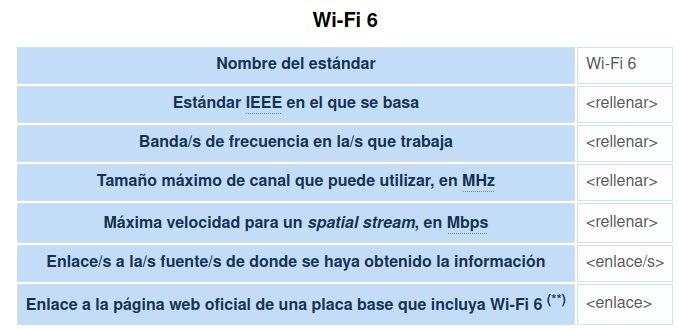
\includegraphics[scale=0.45]{tabla-wifi.png}
    \caption{Tabla a completar con datos de la interfaz Wifi}
\end{figure}

\subsection{Respuesta}

\subsubsection*{Parte 1: Medios Guiados}
En primer lugar vamos a rellenar la tabla con las especificaciones del estándar Ethernet 2.5 Gbs, la información sobre este estándar la hemos recogido de la página de wikipedia \cite{wiki01}, ya que la versión del estándar en la web del IEEE es de pago.

La tabla a quedado así:

\begin{figure}[ht]

    \vspace{3ex}
    \centering

    \setlength{\tabcolsep}{10pt}
    \renewcommand{\arraystretch}{1.4}

    \begin{tabular}{| l | l |}
        \hline
        \textbf{Nombre del estándar}  & 2.5GBASE-T \\ \hline
        \textbf{Estándar IEEE que lo define} & IEEE 802.3bz   \\ \hline
        \textbf{Categoría de cable necesaria para tramo de 100 metros} & Cat 5e   \\ \hline
        \textbf{Ancho de banda de dicho cable} & 100 MHz    \\ \hline
        \textbf{Enlace/s a la/s fuente/s} & \href{https://es.wikipedia.org/wiki/IEEE_802.3bz_(2.5GBASE-T_y_5GBASE-T)}{Wikipedia IEEE 802.3bz}  \\ \hline
        \textbf{Placa Base que incluye Ethernet 2.5G} & \href{https://www.gigabyte.com/Motherboard/Z790-AORUS-XTREME-rev-10/sp#sp}{Gigabyte Z790 AORUS Extreme}   \\ \hline
    \end{tabular}
    \caption{Tabla: Características estándar Ethernet 2.5G}
\end{figure}

\subsubsection*{Parte 2: Medios inalámbricos}
En esta segunda parte vamos a rellenar la tabla con las características del estándar Wifi 6. La información, igual que en el punto anterior, ha sido extraído de la página de Wikipedia relativa al estándar Wifi 6 \cite{wiki02} y la tabla a quedado de la siguiente forma:

\begin{figure}[ht]

    \vspace{3ex}
    \centering

    \setlength{\tabcolsep}{10pt}
    \renewcommand{\arraystretch}{1.4}

    \begin{tabular}{| l | l |}
        \hline
        \textbf{Nombre del estándar}  & Wifi 6 \\ \hline
        \textbf{Estándar IEEE que lo define} & IEEE 802.11ax   \\ \hline
        \textbf{Banda/s de frecuencia en la/s que trabaja} & 2.5GHz, 5GHz y 6GHz \\ \hline
        \textbf{Tamaño máximo de canal que puede utilizar, en MHz} & 160 MHz    \\ \hline
        \textbf{Máxima velocidad para un spatial stream, en Mbps} & 1201 Mbps \\ \hline
        \textbf{Enlace/s a la/s fuente/s} & \href{https://en.wikipedia.org/wiki/Wi-Fi_6}{Wikipedia Wifi 6}  \\ \hline
        \textbf{Placa Base que incluye Wifi 6} & \href{https://www.gigabyte.com/Motherboard/Z790-AORUS-XTREME-rev-10/sp#sp}{Gigabyte Z790 AORUS Extreme}   \\ \hline
    \end{tabular}
    \caption{Tabla: Características estándar Wifi 6}
\end{figure}




% Bibliography

\newpage
\bibliography{citas}
\bibliographystyle{unsrt}

\end{document}